% Created 2021-10-05 Tue 01:07
% Intended LaTeX compiler: pdflatex
\documentclass[11pt]{article}
\usepackage[utf8]{inputenc}
\usepackage[T1]{fontenc}
\usepackage{graphicx}
\usepackage{longtable}
\usepackage{wrapfig}
\usepackage{rotating}
\usepackage[normalem]{ulem}
\usepackage{amsmath}
\usepackage{amssymb}
\usepackage{capt-of}
\usepackage{hyperref}
\author{Ivan Dyachenko}
\date{\today}
\title{\href{https://codeforces.com/edu/course/2/lesson/4}{ITMO Academy. Segment Tree}}
\hypersetup{
 pdfauthor={Ivan Dyachenko},
 pdftitle={\href{https://codeforces.com/edu/course/2/lesson/4}{ITMO Academy. Segment Tree}},
 pdfkeywords={},
 pdfsubject={},
 pdfcreator={Emacs 27.2 (Org mode 9.5)}, 
 pdflang={English}}
\begin{document}

\maketitle
\tableofcontents


\section{Segment Tree}
\label{sec:org2fed6a8}
The segment tree is one of the most useful data structures in competitive programming. For what
tasks is it needed? Let's start with the most basic task.

\subsection{Sum on a segment}
\label{sec:org1544e93}
Suppose we have an array \(a\) of \(n\) elements, and we want to be able to do two operations with
it:
\begin{itemize}
\item \texttt{set(i, v)} - set the element with index \(i\) to \(v\).
\item \texttt{sum(l, r)} - find the sum on the segment from \(l\) to \(r - 1\).
\end{itemize}

Note that in the request for the sum we take the left border \(l\) inclusive, and the right border
\(r\) exclusive. So we will do in all cases when we talk about segments.

\subsection{Structure of the segment tree}
\label{sec:org1cc8885}
Let's imagine that we need to build a segment tree for the following array:
\begin{center}
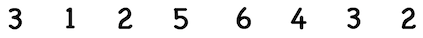
\includegraphics[width=.9\linewidth]{./images/segment-tree-1.png}
\end{center}

The segment tree be constructed as follows. This is a binary tree, in the leaves of which there
are elements of the original array, and each internal node contains the sum of the numbers in its
children.
\begin{center}
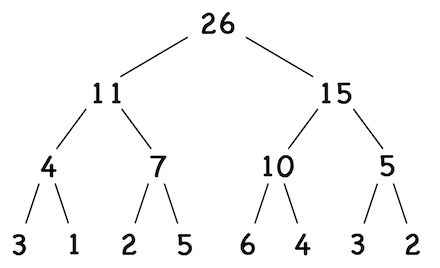
\includegraphics[width=.9\linewidth]{./images/segment-tree-2.png}
\end{center}

Note that the tree turned out so beautiful, because the length of the array was a power of
two. If the length of the array is not a power of two, you can extend the array with zeros to the
nearest power of two. In this case, the length of the array will increase no more than twice, so
the asymptotic time complexity of the operations will not change.

Now let's look at how to do operations on such a tree.

\subsubsection{Operation \texttt{set}}
\label{sec:org4d3446e}
Let's start with the operation \texttt{set}. When the element of the array changes, you need to change
the corresponding number in the leaf node of the tree, and then recalculate the values that will
change from this. These are the values that are higher up the tree from the modified leaf. We
can simply recalculate the value in each node as the sum of the values in children.
\begin{center}
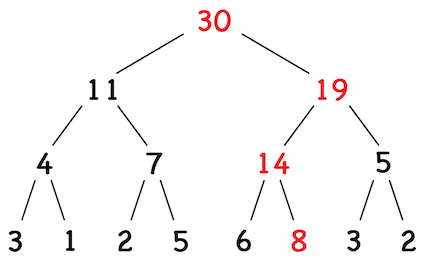
\includegraphics[width=.9\linewidth]{./images/segment-tree-3.png}
\end{center}

When performing such an operation, we need to recalculate one node on each layer of the tree. We
have only \(\log n\) layers, so the operation time will be \(\mathcal{O}(\log n)\).

\subsubsection{Operation \texttt{sum}}
\label{sec:org923d099}
Now let's look at how to calculate the sum on a segment. To do this, let's first see what kind
of numbers are written in the nodes of the segment tree. Note that these numbers are the sums on
some segments of the original array.
\begin{center}
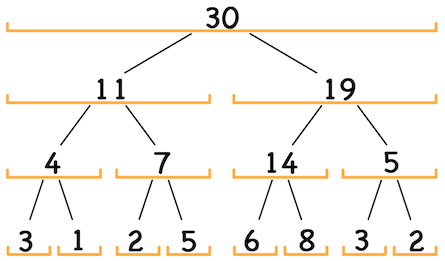
\includegraphics[width=.9\linewidth]{./images/segment-tree-4.png}
\end{center}

In this case, for example, the number in the root is the sum over the entire array, and the
numbers in the leaves are the sum over the segment of one element.

Let's try to build the sum on the segment \([l..r)\) from these already calculated sums. To do
this, run a recursive traversal of the segment tree. In this case, we will interrupt recursion
in two situations:
\begin{itemize}
\item The segment corresponding to the current node does not intersect the segment \([l..r)\). In this
case, all the elements in this subtree are outside the area in which we need to calculate the
sum, so we can stop the recursion.
\item The segment corresponding to the current node is entirely nested in the segment \([l..r)\). In
this case, all the elements in this subtree are in the area in which we need to calculate the
sum, so we need to add to the answer their sum, which is recorded in the current node.
\end{itemize}
\begin{center}
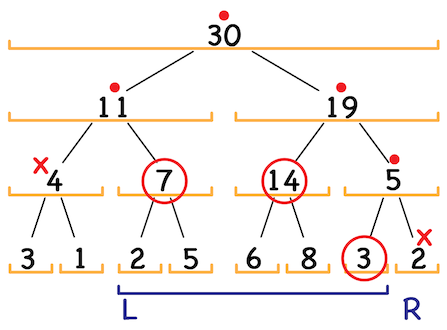
\includegraphics[width=.9\linewidth]{./images/segment-tree-5.png}
\end{center}

Here, the crosses indicate the vertices at which the recursion broke off in the first cutoff,
and the vertices in which the number was added to the answer are circled.

How long does such a tree traversal work? To answer this question, we need to understand how
many nodes none of the cutoffs will happen in, and we will need to go deeper into the tree. Each
such case gives us a new branch of recursion. It turns out that there will be quite a few such
nodes. The fact is that in order for none of the cutoffs to work, the segment corresponding to
the node of the tree must intersect the query segment, but not be contained in it entirely. This
is only possible if it contains one of the boundaries of the segment \([l..r)\). But on each layer
of the tree of segments there can be no more than one segment containing each of the
boundaries. Thus, there can be no more than \(2\cdot\log n\) nodes at which cutoffs did not work,
and, therefore, the general asymptotic time of this procedure will be \(\mathcal{O}(\log n)\).

\subsubsection{Operation \texttt{min}}
\label{sec:orgb50bb00}
What other operations can be done using the segment tree? Instead of the sum, you can calculate
other functions on the interval, for example, a minimum:
\begin{itemize}
\item \texttt{min(l, r)}, which returns the minimum of the segment \(a[l..r - 1]\).
\end{itemize}

How to handle such an operation using the segment tree? Let's build the same tree as for the
sum, only in each node record not the sum of the elements in children, but the minimum.
\begin{center}
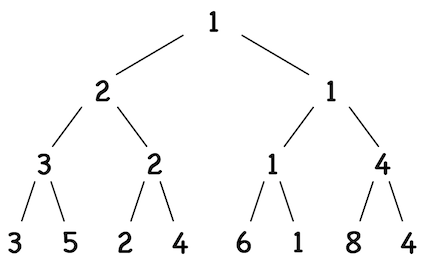
\includegraphics[width=.9\linewidth]{./images/segment-tree-6.png}
\end{center}

The \texttt{set} operation is performed as before. You need to replace the element in the leaf node and
then recalculate the values up the tree to the root. The operation \texttt{min} is performed in the
same way as \texttt{sum}: you need to traverse the tree, while doing the same cutoffs, while the
segment will be divided into several segments, on which we already know the minimum. Talking a
minimum of these numbers, we get a minimum over the entire segment. The operation time will also
be \(\mathcal{O}(\log n)\).

\subsubsection{Other operations}
\label{sec:orgb167519}
In addition to the sum and the minimum, using the segment tree, you can calculate any
associative operation. The operation \(\otimes\) is called \emph{associative} if its result does not
depend on the order in which it is calculated, that is, if \((a \otimes b) \otimes c = a \otimes
    (b \otimes c)\).

For example, in addition to the sum and the minimum, associative operations are:
\begin{itemize}
\item multiplication (including modulo multiplication, matrix multiplication, etc.),
\item bitwise operations,
\item the largest common divisor.
\end{itemize}

In simpler terms, a function can be used for a segment tree, if you know the result of its
calculation for two halves of a segment, you can quickly calculate its result for the entire
segment.

\subsection{Common problems}
\label{sec:org97fc2be}
We learned how to build the segment tree. Let's figure out how to solve the following problems.

\subsubsection{The segment with the maximum sum}
\label{sec:orgbcaac67}
Now we consider the problem of finding a segment with a maximum sum. Our data structure must
support two operations on the array:
\begin{itemize}
\item \texttt{set(i, v)} - set the element with index \(i\) to \(v\).
\item \texttt{max\_segment()} - find the segment of the array with the maximum sum.
\end{itemize}

Let's try to build a segment tree that calculates the required function.

Consider the segment \(x\), which is divided into two halves. We want for the segment \(x\) to find
the value \(seg\): the sum on the subsegment with the maximum sum. Note that knowing only \(seg_1\)
and \(seg_2\) (answers for halves) we cannot get \(seg\), because the answer for \(x\) can intersect
both segments. But in case of intersection, the optimal segment consists of the suffix of the
left half and the prefix of the right half. Let's record for each segment two more values:
\(pref\) and \(suf\) (prefix and suffix with the maximum sum). Then you can calculate \(seg\) as
follows: \(seg = max(seg_1, seg_2, suf_1 + pref_2)\).
\begin{center}
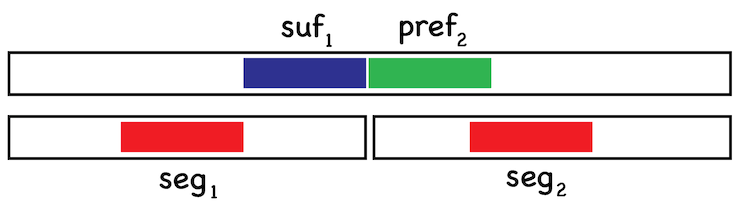
\includegraphics[width=.9\linewidth]{./images/segment-tree-7.png}
\end{center}

Now we need to recalculate \(pref\) and \(suf\). Consider \(pref\), \(suf\) will be considered
similarly. The maximum prefix is either the maximum prefix of the left half, or consists of the
entire left half and the maximum prefix of the right half. Add to each node another value \(sum\),
equal to the sum on the segment. Then \(pref = max(pref_1, sum_1 + pref_2)\), similarly \(suf =
    max(suf_2, sum_2 + suf_1)\). Finally, the sum can be calculated using the formula \(sum = sum_1 +
    sum_2\).

Similarly, we can construct a data structure with the additional operation \texttt{max\_subsegment(l,
    r)}, which find the subsegment of the segment from \(l\) to \(r\) with the maximum sum. To do this,
you need to learn how to merge answers for segments, and this is what we just learned to do.

\subsubsection{K-th one}
\label{sec:org17d1a39}
Consider the problem of finding the \(k\)-th one. Our data structure must support two operations
on the array:
\begin{itemize}
\item \texttt{set(i, v)} - set element \(i\) to \(v \in \{0, 1\}\),
\item \texttt{find(k)} - find the index of the \(k\)-th one.
\end{itemize}

The main idea: we maintain a segment tree with the operation \(sum\). Changing an element is done
in a standard way. Finding the \(k\)-th one is equivalent to finding the leftmost prefix with
the sum \(k + 1\). The algorithm is quite simple. Suppose we need to find the \(k\)-th one on the
segment \([l, r)\). If \(r = l + 1\), then we found the desired one. Otherwise, we look at the sum
\(s\) on the left subsegment. If \(k < s\), then the \(k\)-th one is in the left subtree, otherwise,
we need to start the search for the one with index \(k - s\) in the right subtree.

Obviously, the time of \texttt{find} is \(\mathcal{O}(\log n)\). \\

Consider a small example. We construct a segment tree with the operation \(sum\). And let's get
\texttt{find(3)} query. We start at the root, the segment \([0, 8)\), and search of the third one. We
look at the left subsegment \([0, 4)\) and see that it has a sum of \(2\), which is less than \(k + 1
    = 4\). Therefore, we go down to the right subsegment \([4, 8)\) and look for \(k - 2 = 3 - 2 =
    1\)-th one on it. In the left subsegment \([4, 6)\), the sum is \(2\), which is less than or equal
to \(k + 1 = 1 + 1 = 2\), so our unit lies in the subsegment \([4, 6)\). And finally, in the left
subsegment \([4, 5)\), the sum is \(1\), which is less than \(2\), which means our one is in the right
subsegment \([5, 6)\).
\begin{center}
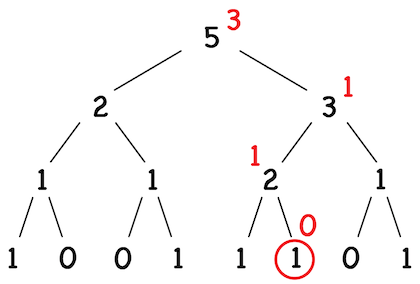
\includegraphics[width=.9\linewidth]{./images/segment-tree-8.png}
\end{center}
\end{document}